\documentclass[fleqn]{jbook}
\usepackage{physpub}

\begin{document}

\begin{question}{専攻 問題2}{}

% Definition of local macros
\def\Iint#1{\int_{-\infty}^{+\infty}\!\!\!{#1}\,}
\def\Isum#1{\sum_{{#1}=-\infty}^{\infty}}

不純物による固体中の電子の束縛問題を考える。簡単のために、格子定数が
 $a$ の一次元結晶とし、格子点は
 $x = na$; $n = 0, \pm 1, \pm 2, \cdots$ で、不純物は $x = 0$ に
あるとする。

\begin{center}
  \mbox{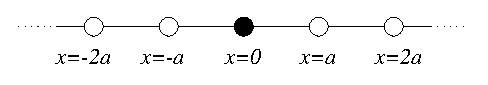
\includegraphics[clip]{1996phy2-1.eps}}
\end{center}

完全結晶の場合に、格子点にあるイオンからのポテンシャルを
 $V_{\rm ion}(x)$ とし、 $x = 0$ にある不純物によるポテンシャル
 $V_{\rm impurity}(x)$ は、$V_{\rm ion}(x)$ に $\Delta V(x)$ が
加わったものとする。
 $V_{\rm ion}(x)$ や $V_{\rm impurity}(x)$ の概略は下図のようであるが、
本問では共にデルタ関数型に簡略化する。

\begin{center}
 \mbox{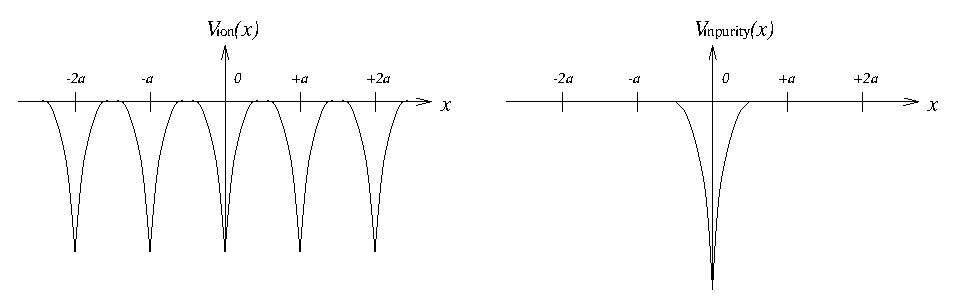
\includegraphics[clip]{1996phy2-2.eps}}
\end{center}



\begin{subquestions}
\SubQuestion
  まず、$V_{\rm ion}(x) \equiv 0$、すなわち、1 次元の自由運動
  をする質量 $m$ の電子が 
  $ \Delta V(x) = -\frac{\hbar^2}{m \lambda_0} \delta (x) $
  によって束縛される問題を考える。 
  ここで、$\lambda_0 > 0$ とする。

  \begin{subsubquestions}
  \SubSubQuestion
    束縛エネルギー $E_0$ の電子の波動関数 $\phi_0(x)$ に対する
    シュレーディンガー方程式を書き下せ。

  \SubSubQuestion
    この方程式にフーリエ変換
    \begin{equation}
        \phi_0(x) = \Iint{\frac{\d{k}}{2 \pi}} e^{-ikx}\phi_0(k)
        \eqname{Q1}
    \end{equation}
    を施し、$k$ 空間でのシュレーディンガー方程式が次のように
    書けることを示せ。
    \begin{equation}
        \frac{\hbar^2 k^2}{2m}\phi_0(k)
      - \frac{\hbar^2}{m \lambda_0} \Iint{\frac{\d{k^\prime}}{2 \pi}} \phi_0(k^\prime)
      = E_0 \phi_0(k)
        \eqname{Q2}
    \end{equation}

  \SubSubQuestion
    $E_0$ を $-\frac{\hbar^2 \kappa^2}{2m}$ と書くと、
    $\phi_0(k)$ は
    \begin{equation}
        \phi_0(k) = \frac{C_0}{k^2 + \kappa ^2}
        \eqname{Q3}
    \end{equation}
    と書ける。ここで、定数 $C_0$ は
    \begin{equation}
        C_0 = \frac{2}{\lambda_0} \Iint{\frac{\d{k}}{2 \pi}} \phi_0(k)
        \eqname{Q4}
    \end{equation}
    である。 式\eqhref{Q3}と 式\eqhref{Q4}とを組み合わせて
    $\kappa$ を求めよ。
    また、$E_0$ を $\lambda_0$ の関数として求めよ。
 
  \SubSubQuestion
    $\phi_0(k)$ のフーリエ逆変換 $\phi_0(x)$ を $\lambda_0$ を
    パラメータとして求めよ。
    そして、$\phi_0(x)$ の概要を図示し、$\lambda_0$ の物理的な意味を
    述べよ。なお、波動関数を規格化する必要はない。

  \end{subsubquestions}
\newpage
\SubQuestion
  次に、$\Delta V(x) \equiv 0$ の完全一次元結晶を考える。すなわち、
  $\lambda > 0$ として、
  \begin{equation}
    V_{\rm ion}(x) = -\frac{\hbar^2}{m \lambda} \Isum{n} \delta(x-na)
    \eqname{Q5}
  \end{equation}
  の場合に、{\bf 1}. に従い、$k$ 空間での電子の波動関数 $\phi (k)$を
  使って固有値問題を解こう。

  \begin{subsubquestions}
  \SubSubQuestion
    エネルギー $\varepsilon$ の電子の $\phi (x)$ を決める
    シュレーディンガー方程式は次のようになることを示せ。
    \begin{equation}
        \frac{\hbar^2 k^2}{2m}\phi(k) 
      - \frac{\hbar^2}{m \lambda a} 
        \Isum{n} \phi(k-\frac{2\pi}{a} n)
      = \varepsilon \ \phi(k)
        \eqname{Q6}
    \end{equation}
    なお、次のポアソンの和公式に注意せよ。
    \begin{equation}
        \Isum{n} e^{inx} = 2 \pi \Isum{n} \delta(x-2\pi n)
        \eqname{Q7}
    \end{equation}

  \SubSubQuestion
    $ \varepsilon = - \frac{\hbar^2 \kappa^2}{2m} $と書くと、
    $ -\frac{\pi}{a} < k < \frac{\pi}{a} $を満たす任意の
    $k$ や整数 $n$ に対して、
    \begin{equation}
        \phi(k - \frac{2 \pi}{a} n) 
        = \frac{C_k}{(k - \frac{2 \pi}{a} n )^2 + \kappa^2}
        \eqname{Q8}
    \end{equation}
    と書ける。 ここで、$k$ にはよるが、$n$ にはよらない数
    $C_k$ は
    \begin{equation}
        C_k = \frac{2}{\lambda a} 
        \Isum{n} \phi(k-\frac{2\pi}{a} n)
        \eqname{Q9}
    \end{equation}
    である。 これから、$\kappa$ と $k$ とは次の関係で結びつく
    ことを示せ。
    \begin{equation}
        \cos(ak) = \cosh(a\kappa) - \frac{1}{\kappa\lambda}\sinh(a\kappa)
        \eqname{Q10}
    \end{equation}
    なお、$u, v > 0$ として、次の公式を使ってもよい。
    \begin{equation}
        \Isum{n} \frac{v}{(n - u)^2 + v^2}
        = \pi \frac{\sinh(2\pi v)}{\cosh(2\pi v) - \cos(2\pi u)}
        \eqname{Q11}
    \end{equation}

  \SubSubQuestion
    式\eqhref{Q10}から、$\lambda <\!\!\!< a$ の場合、
    $ -\frac{\pi}{a} < k < \frac{\pi}{a} $ 
    の範囲の任意の $k$ に対して、$\kappa$ は近似的に
    \begin{equation}
        \kappa = \frac{1}{\lambda} \bigl[ 1 + 2 e^{-a/\lambda} \cos(ak) \bigr]
        \eqname{Q12}
    \end{equation}
    のように与えられることを示せ。

  \SubSubQuestion
    式\eqhref{Q12}から、$k$ の関数としてのエネルギーの固有値
    $\varepsilon_k$ (分散関係)が決められる。
    $ \Norm{k} \ll \frac{\pi}{a} $
    の場合には、それは次の式に示すような自由電子の分散関係に類似した
    形を持つことを示せ。
    \begin{equation}
      \varepsilon_k = \varepsilon_0 + \frac{\hbar^2 k^2}{2m^{\ast}}
      \eqname{Q13}
    \end{equation}
    このとき、 $\varepsilon_0$ や電子の有効質量 $m^\ast$ は
    どのように与えられるか。

  \end{subsubquestions}

\SubQuestion
  最後に、$\Delta V(x) \neq 0$ で $V_{\rm ion}(x) \neq 0$ の場合を
  考える。これまでのように、$k$ 空間でのシュレディンガー方程式から
  出発すると、$x = 0$ にある不純物に捕らえられた電子の束縛エネルギー
  $\bar{E}_0$ が一般的に求められる。しかし、これまでの結果をよく
  考察すれば、次の2つの極限的な場合には $\bar{E}_0$ の値は予測できる。
  その予測値を記し、そのように予測した理由を書け。

  \begin{subsubquestions}
  \SubSubQuestion
    $\lambda \ll a$、且つ、$\lambda_0 \ll a$ の場合。

  \SubSubQuestion
    $\lambda \ll a \ll \lambda_0$ の場合。

  \end{subsubquestions}

\end{subquestions}
\end{question}
\begin{answer}{専攻 問題2}{}
% Definition of local macros 
\def\Iint#1{\int_{-\infty}^{+\infty}\!\!\!{#1}\,}
\def\Isum#1{\sum_{{#1}=-\infty}^{\infty}}
\def\magari{{\frown\kern-.85em\prime\ }}
\def\ucycle{{{\frown\kern-.85em\prime\ }%
\kern-.6em\lower.65ex\hbox{\scriptsize $\rightarrow$}\ }}
\def\dcycle{{{\smile\kern-.85em`\ }%
\kern-.6em\raise.65ex\hbox{\scriptsize $\rightarrow$}\ }}


\begin{subanswers}
\SubAnswer
  \begin{subsubanswers}
  \SubSubAnswer
    $\IDelta V$ のポテンシャル中のエネルギー$E_0$の電子の
    Schr\"{o}dinger方程式は以下の通り。
%
    \begin{equation}
      -\frac{\hbar^2}{2m}\Deriver{^2}{x^2}\phi_0(x)%
      -\frac{\hbar^2}{m\lambda_0}\delta(x)\phi_0(x)%
      = E_0 \phi_0(x) \eqname{A1}
    \end{equation}
%

  \SubSubAnswer
    式\eqhref{A1}の各項の$\phi_0(x)$に式\eqhref{Q1}を代入すると、
%
    \[ %
       \Iint{\frac{\d{k}}{2 \pi}} \frac{\hbar^2k^2}{2m} e^{-ikx}\phi_0(k)%
      -\frac{\hbar^2}{m\lambda_0}%
       \delta(x)\Iint{\frac{\d{k}}{2 \pi}} e^{-ikx}\phi_0(k)
     = E_0 \Iint{\frac{\d{k}}{2 \pi}} e^{-ikx}\phi_0(k) \]
%
    各項に $e^{ik'x}$をかけて$x$で積分すると
%
    \[ \mbox{[第1項]}\Longrightarrow%
        %
        \Iint{\bqquad\d{x}}\Iint{\frac{\d{k}}{2 \pi}} \frac{\hbar^2k^2}{2m}%
        e^{-i(k-k')x}\phi_0(k)%
     =  \Iint{\bqquad\d{k}}\frac{\hbar^2k^2}{2m}\delta(k-k')\phi_0(k)%
     =  \frac{\hbar^2k^{\prime 2}}{2m}\phi_0(k') \]
    \[ \mbox{[第2項]}\Longrightarrow%
       \frac{\hbar^2}{m\lambda_0}%
       \Iint{\bqquad\d{x}}\delta(x)\Iint{\frac{\d{k}}{2 \pi}}%
       e^{-i(k-k')x}\phi_0(k)%
     = \frac{\hbar^2}{m\lambda_0}%
       \Iint{\frac{\d{k}}{2 \pi}} \phi_0(k) \]
    \[ \mbox{[第3項]}\Longrightarrow%
       E_0 \Iint{\bqquad\d{x}}\Iint{\frac{\d{k}}{2 \pi}}%
       e^{-i(k-k')x}\phi_0(k)%
     = E_0 \Iint{\bqquad\d{k}} \delta(k-k')\phi_0(k)%
     = E_0 \phi_0(k') \]
%
    よって式\eqhref{A1}の全体のこの計算の結果は、
%
    \[ \frac{\hbar^2k^{\prime 2}}{2m}\phi_0(k')%
       -\frac{\hbar^2}{m\lambda_0}%
        \Iint{\frac{\d{k}}{2 \pi}} \phi_0(k)%
      = E_0 \phi_0(k') \]
%
    $k,k'$の記号を入れ換えることで式\eqhref{Q2}が示される。


  \SubSubAnswer
    \parbox[t]{100mm}{
    式\eqhref{Q2}で $E_0=-\frac{\hbar^2 \kappa^2}{2m}$とおいて整理することに
    より次式を得る。
%
    \[ \phi_0(k) =%
        \frac{2m}{\hbar^2(k^2+\kappa^2)}\cdot%
        \frac{\hbar^2}{m\lambda_0}\Iint{\frac{\d{k'}}{2 \pi}} \phi_0(k')\]
%
    ここで式\eqhref{Q4}の定義で$C_0$を用いると式\eqhref{Q3}となる。
    式\eqhref{Q4}の$\phi_0(x)$に式\eqhref{Q3}を代入して、$C_0\neq 0$ で
    あるので$ C_0 $で割って整理すると
%
    \[ \lambda_0\pi = \Iint{\d{k}}\frac{1}{k^2+\kappa^2} \]
%
    }\parbox[t]{50mm}{
    \begin{center}
      \mbox{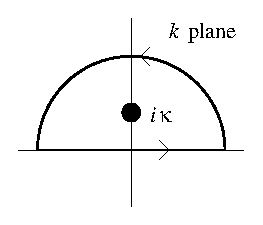
\includegraphics[clip]{1996phy2-3.eps}}
    \end{center}}\\
%
    この積分は右図の経路の複素積分に拡張することができる。
    よって留数定理により
%
    \[ \Iint{\d{k}}\frac{1}{k^2+\kappa^2}%
       = \oint_\ucycle\d{k}\frac{1}{k^2+\kappa^2}%
       = 2\pi i \lim_{k\to +i\kappa}(k-i\kappa)\frac{1}{k^2+\kappa^2}%
       = \frac{\pi}{\kappa} \]
%
   となるので結局
%
    \[ \kappa =  \frac{1}{\lambda_0} \hspace{15mm}%
        E_0   = -\frac{\hbar^2}{2m\lambda_0^2} \]
%
    であることがわかる。

  \SubSubAnswer
    \parbox[t]{100mm}{
    式\eqhref{Q1}の$\phi_0(x)$に式\eqhref{Q3}を代入すると
%
    \[  \phi_0(x)%
        = \frac{C_0}{2\pi}\Iint{\d{k}}\frac{e^{-ikx}}{k^2+\kappa^2} \]
%
    この積分は$x$の正負によって右図のように$2$種の経路の複素積分に
    拡張することができる。よって留数定理により
%
    }\parbox[t]{50mm}{
    \begin{center}\vspace*{-25mm}
      \mbox{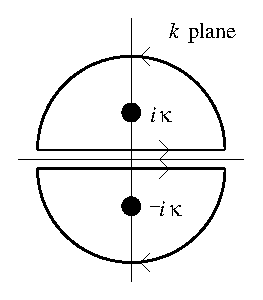
\includegraphics[clip]{1996phy2-4.eps}}
    \end{center}}

\newpage
    \[ \hspace{-5mm}\mbox{($x\ge0$の場合)}\quad%
       \Iint{\d{k}}\frac{e^{-ikx}}{k^2+\kappa^2}%
       = \oint_\dcycle \d{k}\frac{e^{-ikx}}{k^2+\kappa^2}%
       = -2\pi i \lim_{k\to -i\kappa}(k+i\kappa)%
         \frac{e^{-ikx}}{k^2+\kappa^2}%
       = \pi\frac{e^{-\kappa x}}{\kappa} \]
    \[ \hspace{-5mm}\mbox{($x<0$の場合)}\quad%
       \Iint{\d{k}}\frac{e^{-ikx}}{k^2+\kappa^2}%
       = \oint_\ucycle \d{k}\frac{e^{-ikx}}{k^2+\kappa^2}%
       = +2\pi i \lim_{k\to +i\kappa}(k-i\kappa)%
         \frac{e^{-ikx}}{k^2+\kappa^2}%
       = \pi\frac{e^{+\kappa x}}{\kappa} \]
%
    となるので結局
%
    \[  \phi_0(x)%
        = \frac{C_0}{2\kappa} e^{-\kappa |x|}%
        = \frac{C_0\lambda_0}{2} e^{-\frac{|x|}{\lambda_0}} \]
%
    が得られる。$\lambda_0$は波動関数の広がりの程度を表している
    ことがわかる。

    \begin{center}
      \mbox{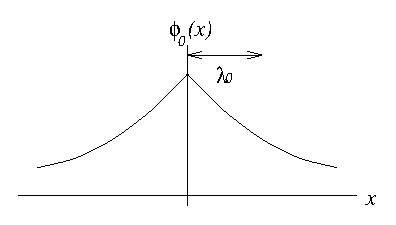
\includegraphics[clip]{1996phy2-5.eps}}
    \end{center}

  \end{subsubanswers}


\SubAnswer
  \begin{subsubanswers}
  \SubSubAnswer
    Schr\"{o}dinger方程式は式\eqhref{A1}と同様に、
%
    \begin{equation}
      -\frac{\hbar^2}{2m}\Deriver{^2}{x^2}\phi(x)%
      -\frac{\hbar^2}{m\lambda}\sum_{n} \delta(x\!-\!na)\phi(x)%
      = \varepsilon \phi(x) \eqname{A2}
    \end{equation}
%
    である。設問{\bf 1}(ii)と同様にフーリエ変換を代入して
    $e^{ik'x}$をかけて$x$で積分する。
    ここで式\eqhref{A2}の左辺第2項についてのこの計算に注目する。
%
    \[ \mbox{[第2項]}\Longrightarrow%
        \frac{\hbar^2}{m\lambda}%
        \Iint{\bqquad\d{x}}e^{ik'x}\sum_n\delta(x\!-\!na)%
        \Iint{\frac{\d{k}}{2 \pi}} e^{-ikx}\phi(k)%
      = \frac{\hbar^2}{m\lambda}%
        \sum_n \Iint{\frac{\d{k}}{2 \pi}} e^{-i(k-k')na}\phi(k) \]
%
    ここで式\eqhref{Q7}のヒントにより、
%
    \begin{eqnarray*}
      \hspace{10mm}%
      &=& \frac{\hbar^2}{m\lambda}%
          \sum_n \Iint{\frac{\d{k}}{2 \pi}}%
          2\pi \delta(-(k\!-\!k')a-\!2\pi n) \phi(k) \\
      &=& \frac{\hbar^2}{m\lambda a}%
          \sum_n \Iint{\bqquad\d{(ak)}}%
          \delta(-ak+ak'\!-\!2\pi n) \phi(k)
       =  \frac{\hbar^2}{m\lambda a}%
          \sum_n \phi(k'-\frac{2\pi}{a}n)
    \end{eqnarray*}
%
    よって式\eqhref{A2}の全体のこの計算の結果は、
%
    \[ \frac{\hbar^2k^{\prime 2}}{2m}\phi(k')%
        -\frac{\hbar^2}{m\lambda a}\sum_n\phi(k'-\frac{2\pi}{a}n)%
        = \varepsilon\phi(k') \]
%
    $k,k'$の記号を入れ換えることで式\eqhref{Q6}が示される。

  \SubSubAnswer
    $\phi$を式\eqhref{Q8},\eqhref{Q9}から消去して $C_k \neq 0$より
%
    \[ 1 = \frac{2}{\lambda a}\sum_n%
           \frac{1}{(k-\frac{2\pi}{a}n)^2+\kappa^2}%
         = \frac{1}{\lambda\pi\kappa} \sum_n%
           \frac{(a\kappa/2\pi)}{(n-(ak/2\pi))^2+(a\kappa/2\pi)^2} \]
%
    を得る。この式は式\eqhref{Q11}のヒントにより、
%
    \[ 1 = \frac{1}{\lambda\kappa}%
           \frac{\sinh{(a\kappa)}}{\cosh{(a\kappa)}-\cos{(ak)}} \]
%
    となる。これより式\eqhref{Q10}が導かれる。

  \SubSubAnswer
    設問{\bf 1}と同様に$\kappa \sim 1/\lambda$ と仮定すれば
    $\lambda \ll a$の条件は $1\sim \lambda\kappa \ll a\kappa$
    となる。この条件のもとで式\eqhref{Q10}を近似すると
%
    \begin{eqnarray*}
      \cos{(ak)} &=&  \frac{e^{a\kappa}+e^{-a\kappa}}{2}%
                     -\frac{1}{\lambda\kappa}%
                      \frac{e^{a\kappa}-e^{-a\kappa}}{2}%
                \sim  \frac{e^{a\kappa}}{2}%
                      \left(1-\frac{1}{\kappa\lambda}\right) \\
    \Yueni \;%
      \kappa &\sim& \frac{1}{\lambda}\cdot%
                    \frac{1}{1-2e^{-a\kappa}\cos{(ak)}}%
              \sim  \frac{1}{\lambda}(1+2e^{-a\kappa}\cos{(ak)})
    \end{eqnarray*} 
%
    この $\kappa$ を再び $e^{-a\kappa}$ の $\kappa$ に代入することで
%
    \[ \kappa \sim \frac{1}{\lambda}%
                   \bigl[1+2e^{-\frac{a}{\lambda}}\cos{(ak)}\bigr] \]
%
    が得られ式\eqhref{Q12}が示された。


  \SubSubAnswer
    $\varepsilon_k$は
%
    \[ \varepsilon_k%
        = -\frac{\hbar^2\kappa^2}{2m}%
        = -\frac{\hbar^2}{2m\lambda^2}%
           \bigl[1+2e^{-\frac{a}{\lambda}}\cos{(ak)}\bigr]^2 \]
%
    である。$ak\ll 1$の条件でこれを$ak$の$2$次まで展開すると、
%
    \begin{eqnarray*}
      \varepsilon_k%
        &\sim& -\frac{\hbar^2}{2m\lambda^2}\bigl[%
                1+2e^{-\frac{a}{\lambda}}(1-\frac{(ak)^2}{2})%
               \bigr]^2 \\
        &=&    -\frac{\hbar^2}{2m\lambda^2}\bigl[%
                 (1+2e^{-\frac{a}{\lambda}})%
                 - e^{-\frac{a}{\lambda}}a^2k^2%
               \bigr]^2 \\
        &\sim& -\frac{\hbar^2(1+2e^{-\frac{a}{\lambda}})^2}%
                {2m\lambda^2}%
               +\frac{\hbar^2k^2(1+2e^{-\frac{a}{\lambda}})e^{-\frac{a}{\lambda}}a^2}{m\lambda^2}
    \end{eqnarray*}
%
    よって式\eqhref{Q13}の形で$\varepsilon_k$が表され、
%
    \[ \varepsilon_0%
       = -\frac{\hbar^2 (1+2e^{-\frac{a}{\lambda}})^2}{2m\lambda^2}
       \hspace{15mm}
       m^\ast%
       = \frac{m\lambda^2 e^{\frac{a}{\lambda}}}%
              {2a^2(1+2e^{-\frac{a}{\lambda}})} \]
%
    と表される。

  \end{subsubanswers}

\SubAnswer
  \begin{subsubanswers}
  \SubSubAnswer
    $\lambda_0$や$\lambda$は電子の広がりを表していると思われる。
    それが格子間隔よりもずっと小さいので、不純物原子にとらえられた
    電子は$x=0$に局在している。よってその電子の振舞いは設問{\bf 1}
    で求めた状況とほぼ同じである。ただしポテンシャルは不純物による
    ものと結晶の$x=a$付近のものによるものの和である。すなわち、
%
    \[ V_{\rm ion}(x) + \Delta V(x)%
       = -\frac{\hbar^2}{m \lambda} \delta (x)%
         -\frac{\hbar^2}{m \lambda_0} \delta (x)%
       = -\frac{\hbar^2}{m \lambda^{\ast}} \delta (x) \hspace{15mm}%
       {\rm where} \quad \frac{1}{\lambda^{\ast}} = \frac{1}{\lambda} + \frac{1}{\lambda_0} \]
%
    よって電子のエネルギーは $\bar{E}_0$は設問{\bf 1}(iii)を参考にして
%
    \[ \bar{E}_0 = -\frac{\hbar^2}{2m\lambda^{\ast 2}} \]
%
    となる。

  \SubSubAnswer
    電子は前問同様に$x=0$の原子に局在しているが、不純物のポテンシャルは
    結晶のそれにくらべて十分小さいので無視できる。よって電子の振舞いは
    設問{\bf 1}で求めた状況とほぼ同じである。ただしポテンシャルは
    結晶の$x=a$付近のものである。よってエネルギーは $\bar{E}_0$は
    設問{\bf 1}(iii)を参考にして
%
    \[ \bar{E}_0 = -\frac{\hbar^2}{2m\lambda^{2}} \]
%
    となる。

  \end{subsubanswers}

\end{subanswers}
\end{answer}


\end{document}
